\subsection{Live Agent Sharing and Dataflow Ablation}
\label{sec:live-profile}

We run OpenCode v2.0.24 against local Qwen3.5-35B-A3B, quantized as
UD-Q4\_K\_XL, on an RTX 5090. Two 16K-context model slots serve two or four
reviewer roles. Each role runs a fresh task session in each of two rounds;
a final session synthesizes their results. The common input is a
\ProfileCorpusKiB\,KiB snapshot of four actual prototype modules.
The harness specifies accepted effects and broad project read scopes.
The model executes source searches, publications, peer reads,
and ledger appends. This measures execution of a known fragment, not natural
plan discovery or independent answer quality.

Two policies use identical allocation bounds, permissions, and CXL locks.
\emph{Scope-only} retains any object that a pending task is authorized to
read. \emph{Dataflow} retains objects named by accepted future effects,
current pins, or session roots. Both reject operations outside the accepted
effects; introducing such a use requires replanning. Each worker-count/policy
pair has three trials in randomized blocks: \ProfileEpisodes{} episodes,
\ProfileSessions{} task sessions, and \ProfileEvents{} recorded operations.
All episodes publish their outputs; \ProfileProtocol{} follow every required
tool step. One scope-only synthesis omits the requested pre-write read of
\texttt{answer}; its CAS publication succeeds. Every attempt is retained.

\textbf{Physical sharing.} All readers resolve the source to the same device
and inode, with every resident payload and mutex page verified on CXL node 1.
A separate three-repeat concurrent mapping probe holds every mapping alive
while sampling PSS. Shared source mappings sum to 64\,KiB with either two or
four workers. Retaining the same source plus per-worker DRAM copies uses
192 and 320\,KiB, respectively. This is a payload-mapping measurement; model,
interpreter, registry, and RPC buffers are outside that PSS sum.

\textbf{Retention.} Payloads use fixed 64\,KiB slots, including unused bounded
output capacity. We integrate allocated payload bytes over the observed task
interval and divide by that interval to obtain average occupancy. Dataflow
actually unlinks dead backing after task namespaces and pins drain; source,
draft, and review objects remain until their accepted readers finish.
Table~\ref{tab:live-retention} reports trial medians. Replaying scope-only
retention on each dataflow trial's own timestamps yields median byte-time
reductions of \ProfileTwoReplaySaving\% and \ProfileFourReplaySaving\%,
separating lifetime decisions from differences in model execution time.
That replay is a capacity calculation, not another latency measurement.

\begin{table}[t]
\centering
\caption{Measured average live CXL payload. Three trials per cell;
64\,KiB slots include unused reserved output space. Registry/lock storage
is accounted separately in the artifact.}
\label{tab:live-retention}
\begin{tabular}{rrrr}
\toprule
Reviewers & Scope-only & Dataflow & Reduction \\
 & KiB & KiB & \\
\midrule
2 & \ProfileTwoScopeKiB & \ProfileTwoGraphKiB & \ProfileTwoSaving\% \\
4 & \ProfileFourScopeKiB & \ProfileFourGraphKiB & \ProfileFourSaving\% \\
\bottomrule
\end{tabular}
\end{table}

\begin{figure*}[t]
\centering
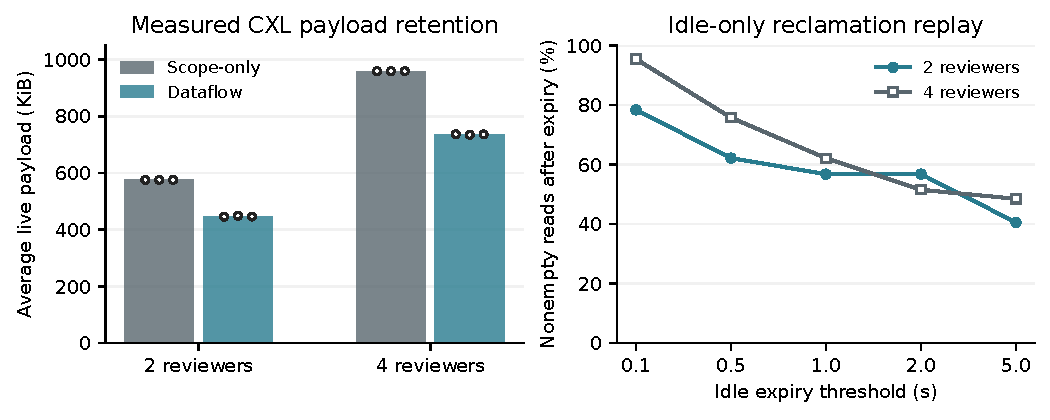
\includegraphics[width=\textwidth]{figures/profile-sharing-profile.pdf}
\caption{Left: measured retention, with median bars and every trial shown.
Right: hypothetical idle-only reclamation replayed on all six dataflow
episodes. A read is at risk when its preceding inter-access gap exceeds the
threshold. No unsafe eviction is executed, and no observed crash is claimed.}
\label{fig:live-retention}
\end{figure*}

\textbf{Why activity alone is insufficient.} With a one-second idle threshold,
\ProfileIdleOneReads{} of \ProfileIdleOneDenominator{} nonempty reads
(\ProfileIdleOnePercent\%) follow an expired interval. This replay counts
future accesses requiring retained or recoverable backing, not actual
use-after-free failures. Scope-only retention is safe but conservative;
idle-only reclamation lacks a future-use guarantee. Object-version dataflow
provides the missing distinction. Equivalent reference tables may provide it
as well. Small prescribed tasks, fixed slot sizes, and two model slots limit
generality. We report no causal inference-speedup or total-process-memory claim.
